\chapter{Aquecimento por indução}
O aquecimento por indução\cite{wiki-induction} é o processo de aquecer um material por meio de indução eletromagnética. As principais causas do aquecimento são as correntes de Foucault e o efeito de histerese magnética. De forma geral, o aquecedor consiste em uma bobina, que é excitada por uma corrente alternada, gerando um campo magnético variável que atua sobre o objeto.

Materiais com permeabilidade magnética relativa baixa, por exemplo, materiais paramagnéticos e diamagnéticos, como o alumínio ou o cobre, são principalmente afetados pelas correntes de Foucault, que são correntes induzidas devido ao campo magnético variável, que, por sua vez, gera uma diferença de potencial no material. Estas correntes, devido à resistência elétrica do material, dissipam calor por efeito Joule, aquecendo do material. Quanto maiores a condutividade do condutor e a intensidade e frequência do campo eletromagnético, maior serão as correntes no material.
\section{Efeito skin}
Em casos de frequências muito elevadas do campo eletromagnético, não há penetração completa do campo no interior do material. Este é chamado o efeito skin, já que as correntes tendem a se concentrar nas bordas do material. Neste caso, a distribuição da corrente não pode mais ser considerada uniforme, e a redução da superfície efetiva do material faz com que a resistência aumente. Sabendo que a potência $P$ pode ser calculada por $P = RI^2$, onde $R$ é a resistência do material e $I$ é a corrente, vemos que a potência dissipada irá aumentar, já que, além do aumento da resistência, a corrente também irá aumentar, apesar da distribuição não uniforme do campo.
\section{Histerese}
A histerese é a tendência de um material de conservar suas características na ausência do estimulo que as gerou. A histerese magnética caracteriza-se pelo fato da densidade do fluxo magnético continuar presente no material mesmo após a intensidade do campo chegar a zero, como podemos ver na \autoref{fig_histerese}. Isto se deve ao fato dos dipolos magnéticos do material tenderem à se alinhar ao campo, e permanecerem assim mesmo após o campo ter cessado.
Em materiais com permeabilidade magnética alta, materiais ferromagnéticos como o ferro, a histerese magnética é o principal gerador de calor em potências mais baixas. A perda por histerese é causada pelo atrito dos dipolos ao se alinharem com o campo magnético. Como o campo magnético varia de acordo com a corrente na bobina, o contínuo realinhamento dos polos com o campo causa, por meio da perda de histerese, o aquecimento do material.

\begin{figure}[h]
\caption{\label{fig_histerese}Curvas de histerese}
\begin{center}
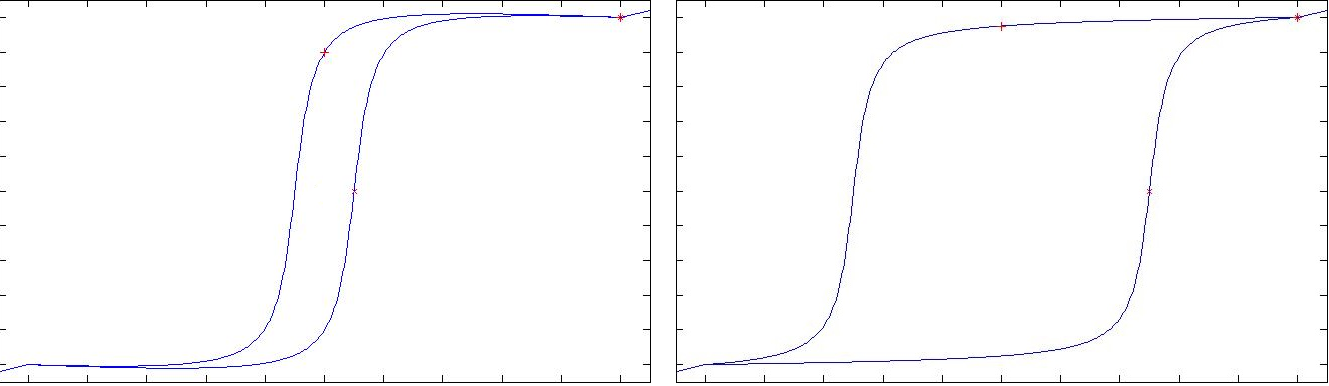
\includegraphics[scale=0.5]{images/histerese.png}
\end{center}
\legend{Curva de magnetização para material com pouca e muita histerese, respectivamente.}
\end{figure}